%\section{Arbeitskultur}
	\section{Einleitung}
Bevor die Wichtigkeit der Arbeitskultur für die Beratungsdienstleistung erläutert wird, wird an dieser Stelle auf die Definition der Arbeitskultur eingegangen. Reinhard Kößler definiert den Begriff der Arbeitskultur im ``Lexikon zur Sozialogie`` von Wernern Fuchs-Heinritz als Verschiedenheit von Visionen des Arbeitsverhaltens in Form von Lebensformen, Einstellungen und Reaktionen auf die Anforderungen der Arbeit in industriell-kapitalistischen Gesellschaft. \cite{Fuchs-HeinritzLautmannRammstedtWienold1994}.
Arbeitskultur ist in der ersten Linie eine Teilmenge der Kultur (Sitten, Bräuche, Mentalität usw.) einer Nation. Gemäß Carsten Weigelt bedeutet die Arbeitskultur für die jungere Generation - sogenannten ``Digital Natives`` viel mehr als Geld und Karriere. Unter Arbeitskultur wird von ihnen das Wohl im Privatleben und am Arbeitsplatz verstanden.
Viel wichtiger ist an dieser Stelle, anstatt dem Begriff von Fuchs-Heinritz, die letzte Definition der Arbeitskultur von ``Digital Natives``zu betrachten. Denn für den Beratungsprozess ist es viel sinnvoller die gewünschte und die gute Arbeitskultur zu betrachten. Um festzustellen was eine gute Arbeitskultur für die IT-Beratung im internationalem Kontext ist, wurden einige Teilaspekte der Arbeitskultur definiert und abschließend werden diese Teilaspekte anhand von ausgewählten Ländern verglichen. Was beeinflusst die gute Arbeitskultur? welche Faktoren führen zum Wohl im Privat-und Berufsleben? Ist es überhaupt wichtig die fremde Arbeitskultur zu analysieren, wenn man international agiert? In wieweit sind die Beratungsdienstleistung von der Arbeitskultur abhängig? Diese und weitere Fragen rund um IT-Beratung, sowie Arbeitskultur im internationalem Kontext werden in den nächsten Abschnitten geklärt. Es werden auch einige Probleme rund um die Arbeitskultur, IT-Beratung und den internationalen Aspekt der Arbeitskultur erläutert.\\
Die Arbeitskultur gehört zum Beratungsprozess und spielt dabei nicht die unwesentlichste Rolle. Welche Arbeitskultur gehört zum Beruf des IT-Beraters? Ein IT-Berater ist immer in der Bewegung und sein Arbeitsplatz ist nicht nur im Büro, sondern auch im Zug, im Restaurant oder im Auto. Es ist sehr ersichtlich, dass die Arbeitskultur des Beraters mit der Arbeitskultur von Kunden des Beraters unzertrennlich ist. IT-Consultans lernen innerhalb der wenigsten Zeit sehr viele Firmen und deren Mitarbeiter kennen. An dieser Stelle stoßen die IT-Berater auf unterschiedlichste Arbeitskulturen. Berater arbeiten oft durch Kommunikation mit Menschen aus unterschiedlichen Unternehmensebenen (Mitarbeiter, Manager, Geschäftsführer usw.), verschiedenen Branchen (Finanzdienstleistung, Fahrzeugbau, Großhandel, Chemieindustrie usw.) oder in unterschiedlichen Länder mit jeweils einzigartigen Kulturen und damit auch einzigartigen Arbeitskulturen.\\
Im Vergleich zu einem Mechatroniker, der nur eine Arbeitskultur ``kennt``, werden die IT-Berater mit unterschiedlichsten Arbeitskulturen konfrontiert, häufig auch international.\\
Um die Bedeutung der Arbeitskultur im internationalem Kontext für den Beratungsprozess näher zu erläutern, werden an dieser Stelle 2 Beispielfälle erklärt.\\
	 \\
	 a) Der 1. Fall ist ein IT-Consulting-Unternehmen mit eingestellten Beratern, die aus unterschiedlichen Ländern kommen, unterschiedliche Sprachen sprechen und sich kulturell enorm unterscheiden. Wichtig für die Arbeitskultur an dieser Stelle ist es ein kulturelles Gleichgewicht herzustellen und dauerhaft zu behalten. Diese Berater arbeiten zielgerichtet und ständig im Team. Im 1. Fall ist es vor allem  interessant, inwieweit sich kulturellen Unterschiede auf das gemeinsame Ziel des Beratungsprozesses bei der Softwareeinführung auswirken können. Auch interessant ist hier, wie die IT-Berater aus unterschiedlichen Länder mit Kunden aus Deutschland umgehen und ob die kulturelle Unterschiede einen Einfluss auf Kundenbeziehungen haben. \\
	 \\
	 b) Der 2. Fall bezieht sich auf ein deutsches Unternehmen, das international agiert und Kunden aus unterschiedlichen Länder betreut. In diesem Fall müssen sich deutsche Mitarbeiter auf unterschiedliche Arbeitskulturen anpassen. Denn ein Meeting während des Mittagsessen in Japan ist widersinnig und wirkt unseriös. In Japan hat das Essen einen unverletzlichen Status, in USA dagegen ist es nicht ungewöhnlich, dass beim Essen wichtige Entscheidungen kollaborativ getroffen werden.\\
	Wegen der zeitlichen sowie thematischen Begrenzung wird in dieser Arbeit der Fokus nicht auf die Differenzierung dieser zwei Fälle oder auf kulturelle Unterschiede der Berater gelegt, sondern nur auf die unterschiedliche Arbeitskulturaspekte, die für den Beratungsprozess ausschlaggebend sind. Teilaspekte der Arbeitskultur, die für das IT-Consulting als relevant erachtet werden, werden in folgenden Kapiteln vorgestellt und verglichen. In der weiteren Arbeit werden diese zwei Fälle nicht unterschieden und nur im Hintergrund behandelt.
	Diese sind aber wichtig, um zu zeigen, warum sich die IT-Berater-Arbeitskultur nicht nur auf die deutsche Arbeitskultur bezieht, sondern auch im Beratungskontext einen internationalen Charakter hat.\\
	\\
\textbf{Allgemeine Arbeitsabläufe des IT-Consultings}\\ \\
	Nachdem die Arbeitskultur erklärt wurde, werden in diesem Kapitel allgemeine Abläufe des IT-Consultings detaillierter betrachtet. An dieser Stelle ist es unvermeidbar den Beratungsprozess exemplarisch zu zeigen, um die Feinheiten des Prozesses zu verstehen, die von der Arbeitskultur beeinflusst werden, um im Endeffekt Einschlüsse auf die Faktoren der Arbeitskultur zu bilden.\\ 
	IT-Consulting ist eine wichtige Art des Consultings in IT-Fragen eines Unternehmens. Das Wesen des IT-Consultings besteht im Allgemeinen darin, Unternehmen bei der Neustrukturierung der Anwendungslandschaften oder bei der Pflege der bestehenden Informationssysteme zu unterstützen. Während des gesamten Beratungsprozesses bleibt der Berater als externer Experte solange im Unternehmen bis die Probleme, die er mit seinem technischen Fachwissen zu lösen hat, nicht mehr existieren oder selbständig von den Mitarbeitern des Unternehmens gelöst werden können.\\
	Um den Beratungsprozess zu verdeutlichen wird nacholgend ein Beispielprozess aus der Praxis der IT-Beratung beschrieben. \\ Ein Online-Handelsunternehmen möchte ein BI-Standardsoftware einführen und die Daten für Analysezwecke aus dem bestehenden ERP-System laden, um die Kunden zu erkennen, die möglicherweise bald kündigen oder sich für Werbung von neuen Produkte eignen. Am Anfang jedes Prozesses muss dem Berater die Organisationsstruktur und die Geschäftsprozessabläufe des Unternehmens klar sein, um eine passende Lösung zu finden. Das IT-Beratungsunternehmen hat eine Standardsoftware im Einsatz, um die geschäftlichen Probleme eines Unternehmens mit Hilfe von Informationstechnologie zu lösen. Es gibt aber keine Standardlösung die für alle Unternehmensstrukturen passend ist, weil die Unternehmensstrukturen meistens heterogen sind. Nach dem erfolgreichen Vertragsabschluss zwischen Unternehmen und der Consultingfirma beginnt die Analysephase des Beratungsprozesses. Hier wird die Unternehmensstruktur des Online-Handelsunternehmen analysiert, bis man erkennt, wo die Software eingesetzt werden kann. Wichtige Aufgaben bestehen darin, Stellen wo Reibungen entstehen können zu finden, zu ermitteln welche Ressourcen zur Verfügung stehen und zu bestimmen, welches Informationssystem sich am besten für den Unternehmenszweck eignet. Es muss außerdem ein ständiges Feedback zwischen dem Berater und Projektleiter möglich sein.\\
	Nachfolgend wird der Ablauf des Beratungsprozesses intensiver beschrieben. Nach der Analysephase beginnt man der Konzepterstellung, indem für die Ideen und Pläne ein geeignetes Konzept erstellt wird. In der Folge beginnt die Umsetzungsphase, in welcher eine neue IT-Architektur aufgebaut oder die vorhandene ergänzt wird. Im unseren Beispiel wird die ERP-Lösung mit der BI-Lösung erweitert, die vorhandene Architektur bleibt erhalten. In dieser Phase können auch die andere Berater aufgerufen werden, falls es viele komplizierte Realisierungsmaßnahmen gibt.
	Nachdem das Informationssystem erfolgreich in die Unternehmensstruktur integriert ist, beginnen die Schulungsmaßnahmen, damit die Mitarbeiter des Unternehmens in der Lage sind mit diesem System umgehen zu können. Zum Schluss erfolgt die Wartungsphase und Intensität der Beratungsdienstleistung nimmt langsam ab. Diese Prozesskette kann in Form eines Lebenszyklus stattfinden.\\
	Diesen Ablauf kann man graphisch am folgenden Modell des ganzheitlichen Beratungsprozesses erkennen(siehe Abb. 5.1). Dieses Modell liefert uns die einzelnen Phasen der Beratungsdienstleistung eines Freelancers in dem Umfeld der Managementberatung \cite{MngmBerPhasen}.


\begin{figure}[htp]
\centering
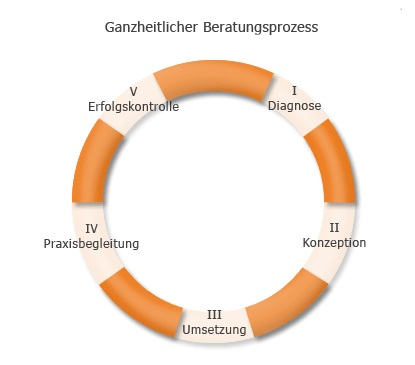
\includegraphics[width=0.7\linewidth]{./images/beratungsproz}
\caption{Phasen des Beratungsprozesses eines Managementberaters, \cite{PhasenBeratungsprozess} }
\label{fig:beratungsproz}
\end{figure}
	
	\textbf{ Bedeutung der Arbeitskultur für IT-Consulting}\\ \\
	In wie weit ist es wichtig die Arbeitskultur für den Beratungsprozess zu betrachten? Anhand vom unseren Beispiel ist zu erkennen, dass die IT-Berater in jeder Phase der Softwareeinführung mit den Unternehmensvertretern kommunizieren sollen. Es ist wichtig, dass die Berater genug technisches Know-how mitbringen. Noch wichtiger sind die Soft Skills, die für erfolgreiche Geschäftsbeziehungen entscheidend sind. ``IT Business is People's Business``. Damit wird gemeint, dass der Erfolg von IT-Projekten sowohl von vertrauensvollen Verhandlungen als auch maßgeblich von der Kompetenz des Beraters abhängt. \cite{ITConsRu}
	Welche sozialen Fähigkeiten sind z.B. für einen us-amerikanischen IT-Berater besonders wichtig? Sind diese persönlichen Eigenschaften auch für die anderen Nationen von der Bedeutung? Unternehmensführung und IT-Berater müssen bei der Lösung des Problems einig werden. Der Berater muss ein Unternehmen für seine vorgeschlagene Lösung überzeugen. Muss man, um das Unternehmen zu überzeugen, nur eine gute Software anbieten und als vertrauenswürdiges Unternehmen am Markt agieren oder reichen diese Bedingungen beispielsweise in Indien nicht aus, weil der Berater möglicherweise aus anderer Kaste ist. Denn die Kastenzugehörigkeit hat in Indien bis heute kulturelle und soziale Auswirkungen auf viele Lebensbereiche \cite{KastensystemInd}.

	Für diese Arbeit ist wichtig zu wissen, wie die Arbeitskultur in ausgewählten Länder sich unterscheidet und in wie weit diese den Beratungsprozess beeinflussen kann.
	In den folgenden Kapiteln wird Arbeitskultur von ausgewählten Ländern (Russland Japan, USA, Deutschland) untersucht und zum Schluss werden einige interessante Fakten verglichen und diskutiert. 
\section{Teilaspekte}
	In diesem Kapitel werden die Teilaspekte der Arbeitskultur von ausgewählten Ländern vorgestellt. Dazu wird eine Matrix, die Länder mit zugehörigen Teilaspekten definiert, aufgestellt. Einige Teilaspekte werden in den nächsten Abschnitten detaillierter beschrieben, um die Wichtigkeit dieser Aspekte für das IT-Consulting hervorzuheben. Andere Teilaspekte, zu denen es nicht genug Information gibt, haben den Forschungsbedarf. Am Ende des Kapitels ``Arbeitskultur``werden einige informationsreiche und interessante Teilaspekte länderspezifisch verglichen, um Rückschlüsse auf die Arbeitskultur im IT-Beratungsgeschäft zu ziehen. 
	Die Recherche zu den Teilaspekten findet in 3 Sprachen (Deutsch, Englisch und Russisch) statt, um den Fokus der Recherche zu verbreiten.
	
\begin{table}[htp]
\begin{tabular}{|c|c|c|c|c|c|}
\hline  Aspekt/Land& Deutschland & USA & Russland & Japan & Indien \\ 
\hline 	Hierarchien  & z & ja & ja & ja &  z \\
\hline  Gehalt& ja & ja & ja & ja & z \\ 
\hline  Gesetze& x & ja & ja & ja & z  \\ 
%\hline  Grad des intuitiven Handelns& ? & ? & ? & ? & ? & ? \\ 
\hline  Kritikfähigkeit& z & z & z & ja & z \\ 
\hline  Team& ja & ja & ja & ja & z\\ 
\hline  Entscheidungsfindung& x & x & ja & ja & z  \\ 
\hline  Lebensstandard& ja & ja & ja & ja & z \\ 
\hline  Pünktlichkeit& ja & z & ja & ja & z\\ 
\hline  Arbeitszeit, Urlaub, W-L-B& ja & ja & ja & ja & z\\ 
\hline 
\end{tabular} 
\caption{Matrix der Arbeitskultur}
\end{table}
Um diese Matrix richtig verstehen zu können, muss man zuerst die einzelnen Symbole definieren. Das Symbol ``Ja`` bedeutet, dass die Information über dem Teilaspekt bezüglich der IT-Beratung im internationalem Kontext vorhanden ist und man daraus einen Vergleich über den gleichen Teilaspekt in ausgewählten Ländern machen kann. Das ``x`` bedeutet, dass man entweder die Information nicht vollständig hat oder, dass es keine eindeutige Beziehung zum unseren Thema gibt. Beispielsweise gibt es genug Information zu den deutschen Gesetzten, trotzdem gibt es hier keine Besonderheit, die den Beratungsprozess in maßgeblicher Weise beeinflusst. Das ``z`` bedeutet, dass aus zeitlichen Gründen keine Information gefunden wurde. Dazu gibt es mehrere Gründe wie bspw. die zeitliche Begrenzung des Projekts, sowie knappe Ressourcen in Form von Projektmitgliedern. Ein weiterer Grund besteht darin, dass es wichtiger war,  Prioritäten zu setzen und die Teilaspekte mit erhöhter Relevanz detaillierter zu betrachten. Aus diesem Grund wird auch das Land Indien nicht erläutert, wie es geplant wurde.\\ \\
%\begin{table}[htp]
%\begin{tabular}{|c|c|c|c|c|c|}
%\hline  Aspekt/Land& Deutschland & USA & Russland & Japan & Indien \\ 
%\hline 	Hierarchien  & ? & ? & ? & ? & ? \\ 
%\hline  Gehalt& ? & ? & ? & ? & ? \\ 
%\hline  Gesetze& ? & ? & ? & ? & ?  \\ 
%%\hline  Grad des intuitiven Handelns& ? & ? & ? & ? & ? & ? \\ 
%\hline  Kritikfähigkeit& ? & ? & ? & ? & ? \\ 
%\hline  Team& ? & ? & ? & ? & ?\\ 
%\hline  Entscheidungsfindung& ? & ? & ? & ? & ?  \\ 
%\hline  Lebensstandard& ? & ? & ? & ? & ? \\ 
%\hline  Pünktlichkeit& ? & ? & ? & ? & ?\\ 
%\hline  Arbeitszeit, Urlaub, W-L-B& ? & ? & ? & ? & ?\\ 
%\hline 
%\end{tabular} 
%\caption{Matrix der Arbeitskultur}
%\end{table}
%Ende der Recherche-> Information für neue Matrix
%1)Hierarchien und Organisation->Hierarchien 2)Kundenverh weg 3)spezielle Rechtslage->Gesetze 4)Grad des intuitiven Handelns weg 5) Kritikfähigkeit nur bei Japan,De 6) Lebensumstände ->Lebensstandards ->Zeitmanagement in Form von Pünktlichkeit 7)Work-Life-Balance-> Arbzeit und Urlaub 8)Entsch.findung nur Russland
%Durch einer Recherchewerden einige Teilaspekte verändert. Dafür gibt es mehrere Gründe, bspw. waren die recherchierten Teilaspekte besser formuliert oder einige waren in ihrer Definition zu weit gefasst und müssten demzufolge zusammengefasst werden. Für bestimmte Teilaspekte gibt es keine Information, die durch Recherche in 3 verschiedenen Sprachen (Deutsch, Englisch und Russisch) nicht zu finden ist. An dieser Stelle besteht noch Forschungsbedarf. 
Dieses Kapitel hat im Vergleich zu den Kapiteln ``Markt`` und ``Bildung`` eine andere Struktur, indem nicht nach den Teilaspekten der Arbeitskultur gegliedert wird. Dafür wird hier eine Unterteilung des Kapitels nach Ländern vorgenommen und in diesen werden die Teilaspekte wie Hierarchien, Gesetze oder Team beschrieben.
Bevor die ausgewählten Ländern untersucht werden, definiert man in folgenden Kapiteln zuerst die wichtigsten Teilaspekte der Arbeitskultur.
\subsection*{Gehalt}
Gehalt ist einer der wichtigsten Faktoren für die angenehme Arbeitskultur. Diejenigen, die ein gutes und faires Gehalt bekommen sind motiviert, meist zufrieden mit ihrem Job und aus psychologischer Sicht sind sie sicher, dass sie für eigene Mühe ein gerechtes Gehalt bekommen. Demzufolge hat das Geld nicht nur die Tauschmittel-Funktion (es erlaubt uns, das zu kaufen, was wir zum Leben brauchen), sondern auch eine psychologische. Laut Täubner steht das Geld für Erfolg, Sicherheit, Anerkennung, Macht, Lebensqualität und Selbständigkeit \cite{GehaltBedeutungDE}.\\
Wenn die Arbeitnehmer im Gegensatz zum guten Verdienst mit ihrem Gehalt unzufrieden sind, dann gibt es meist kein Wohl am Arbeitsplatz. Es lässt sich doch sagen, dass das Geld nicht der wichtigste Faktor für gute Arbeitskultur ist. Laut der StepStone-Studie,in der rund 18.500 Fach- und Führungskräfte befragt wurden, um zu wissen was die Arbeitnehmer am meisten motiviert, steht das Geld nur auf dem 3.Platz nach dem guten kollegialen Arbeitsumfeld und dem Spaß am Arbeiten \cite{GehaltNR.3DE}.\\
 Schlussendlich lässt sich sagen, dass das Gehalt ein wichtiger Motivierungsfaktor ist, der allein zu schwach ist, um eine gute Arbeitskultur zu gewährleisten.
IT-Berater sind daher keine Ausnahme, wenn es um Gehalt geht. Berater arbeiten viel und möchten dafür auch entsprechend entlohnt werden. Die Arbeitszeiten von IT-Berater werden im nächsten Kapitel vorgestellt.\\
Interessant zu wissen ist noch, wie sich das Gehalt von IT-Beratern in den ausgewählten Ländern sich unterscheidet und in wieweit er deren Arbeitskultur beeinflusst.
\subsection*{Arbeitszeit, Urlaub, Work-Life-Balance}
Flexible Arbeitszeiten und viele Urlaubstage sind die wichtigsten Faktoren um die Work-Life-Balance zu bestimmen. Dazu zählen noch laut Feddersen: die Möglichkeit im Homeoffice zu arbeiten, Zeit für Fortbildung und Kinderbetreuung \cite{WLB}.\\
Work-Life-Balance ist heute kein leerer Begriff mehr. Das, was dahinter steht, gewinnt zunehmend an Bedeutung. Arbeitnehmern sowie Arbeitgebern wird immer bewusster, dass die Work-Life-Balance nicht nur die Balance zwischen Job und Privatleben, sondern auch ein wichtiger wirtschaftlicher Faktor ist. Die Work-Life-Balance beeinflusst die Arbeitskultur und auch die Arbeitsleistung sowie die Produktivität von Mitarbeitern, was für Arbeitgeber entscheidend ist, um das Gleichgewicht zwischen Berufs- und Privatleben für die Angestellten zu gewähren. Die Vorbeugung von Burnout-Erkrankungen ist dabei sicherlich ein weiterer, positiver Nebeneffekt. \cite{WLB} \\
Das Gleichgewicht zwischen Berufs- und Privatleben herzustellen, ist für IT-Berater nicht einfach. Denn IT-Berater sind ständig auf Reisen, arbeiten 60-70 Stunden pro Woche und diese Arbeit ist meist geistig  sehr anstrengend \cite{WLBbeiIT-Berater}. Für junge IT-Berater könnte es kein Problem sein, wie sieht es aus wenn man eine Familie und Kinder hat? Laut Robert Laube, der für Service Line ``Business Intelligence`` bei Avanade verantwortlich ist, erfordert die Work-Life-Balance sehr viel Selbstdisziplin \cite{WLBbeiIT-Berater}. Dazu gehört beispielsweise die Verbannung von E-Mails auf dem Handy oder ``[...] morgens mit den Kindern zu frühstücken und sie in die Schule und den Kindergarten zu bringen``, falls es die Zeit erlaubt \cite{WLBbeiIT-Berater}.
\subsection*{Lebensstandard}
Der Lebensstandard in den ausgewählten Ländern gehört auch zum wichtigen Teilaspekt der Arbeitskultur. Es ist vor allem wichtig das Gehalt von IT-Berater im Bezug zum Lebensstandard in einem bestimmten Land zu betrachten. Mit anderen Wörtern kann man den Lebensstandard als Ergänzung zum Gehalt oder als Ergänzung zu der Währung sehen, um das Gehalt in den ausgewählten Ländern objektiver zu vergleichen. An dieser Stelle ist es sinnvoll ein Beispiel zu erwähnen, um den Sachverhalt zu verdeutlichen. IT-Berater aus Deutschland verdienen durchschnittlich mehr als ihre russischen Kollegen, doch sind die Lebenshaltungskosten wie Nahrung, Miete, Kleidung in Russland geringer als in Deutschland.\\
Im Allgemeinen beschreibt der Lebensstandard den sozio-kulturellen Wohlstand von Personen im Verhältnis zu Vergleichspersonen innerhalb einer kulturellen Gemeinschaft. Bestimmt wird dazu die jeweilige Höhe der Lebensbedingungen bzw. die Befriedigung von materiellen und geistig-kulturellen Bedürfnissen. \cite{LbsWiki} \\
Natürlich unterscheiden sich die Faktoren, die den Lebensstandard in den ausgewählten Ländern beeinflussen. Hauptaugenmerk liegt jedoch darauf, wie der Lebensstandard und das Gehalt die Arbeitskultur von IT-Beratern beeinflusst, und nicht auf den internationalen Unterschied von einzelnen Lebensstandardindikatoren.
\subsection*{Team}
IT-Berater arbeiten nicht selten in einem Team zusammen. Die Teamfähigkeit ist eine der wichtigsten sozialen Fähigkeiten des Beraters. Bei der Teamarbeit geht es um eine effiziente Kooperation, dabei bringt jedes Teammitglied seine persönliche Stärken mit ein, damit ein gemeinsames Ziel erreicht werden kann. Es ist daher ersichtlich, dass ein Team mit seiner Struktur eine große Rolle für die IT-Beratung einnimmt.\\
Es ist außerdem aufschlussreich, die Besonderheiten des Teams, sowie die Teamarbeit zum Beispiel die Beziehungen zwischen den einzelnen Teammitgliedern, oder das Ziel der Teamarbeit, in den ausgewählten Ländern zu untersuchen.
\subsection*{Hierarchie}
Unter dem Teilaspekt Hierarchie wird die Geschäftshierarchie gemeint. Die Geschäftshierarchie bestimmt, wie die Geschäftsstruktur aufgebaut ist. Dabei werden meist die Aufgaben, Positionen, sowie Mitarbeiterrollen definiert. Eine gut strukturierte Hierarchie bietet Vorteile für das Unternehmen. Die flache Hierarchie bietet den Mitarbeitern meist mehr Eigeninitiative und –verantwortung beim Ausführen unterschiedlicher Aufgaben. Dabei hat der Ranghöhere wenige Eingriffe in  Entscheidungen von den Rangniedrigeren.
Zu diesem Thema gehören noch solche Faktoren, wie die Entscheidungsfindung bei Mitarbeitern, Kommunkation zwischen Mitarbeitern aus gleichen sowie verschiedenen Unternehmensebenen.\\
Da es sehr wenig Information über der Geschäftshierarchie im IT-Consultingbereich gibt, bezieht sich dieser Teilaspekt nicht nur auf IT-Consulting-Unternehmen, sondern auch auf alle anderen Unternehmen. 
\subsection*{Pünktlichkeit}
Der Pünktlichkeit hat teilweise eine hohe Bedeutung zuteil. In diesem Aspekt wird auch die termingerechte Erfüllung eines Planes im Consultingbereich definiert.  Letzteres  ist sehr wichtig zu betrachten, weil dieser Teilaspekt einige Unterschiede in den ausgewählten Ländern aufweist. Diese Unterschiede können in bestimmten Umständen zu den zeitlichen Verzögerungen von Projekten und damit verbundenen finanziellen Problemen führen.
\section{Analyse der ausgewählten Teilaspekte}
	\subsection*{Russland}	
	\textbf{Einleitung}\\ \\
	Der Aspekt-Markt spielt für die Arbeitskultur ebenfalls eine wichtige Rolle. Zwischen diesen Aspekte gibt es einige Zusammenhänge, wie das Gehalt oder die Arbeitszeiten von IT-Beratern.\\
	Russland ist ein Wachstumsmarkt mit Zukunft. Laut Holger Hirsch ist heute der damals geschützte russischer Markt offen für Exporte und Investitionen aus Deutschland. Dies gilt sowohl für IT-Beratungs-Unternehmen, die ihre Softwareprodukte in Russland integrieren auch für russische Manager, die bei der Informationstechnologie auf westliches Know-how setzen.\cite{ITConsRu}\\
	Da der Markt für IT-Beratung neu ist, muss man als IT-Berater aus Westen ganz viele Entscheidungen intuitiv treffen. Hier werden natürlich die Soft Skills des Beraters gefragt. Technische Fähigkeiten, funktionales Wissen und Branchen-Know-how sind selbstverständlich vorausgesetzt. ´´Der Zerfall der Sowjetunion und die Reformen im wirtschaftlichen und sozialen Gefüge Russlands haben einen erheblichen Einfluss auf die Arbeitskultur in gegenwärtigen russischen Organisationen´´\cite{ProzessbeglBerRU}.
	Deswegen überlappen sich die kulturellen- mit reformbedingten Faktoren der Arbeitskultur. Es ist daher sehr schwer den Ursprung dieser Faktoren zu unterscheiden. Am Beispiel des russischen Kollektivs könnte diese Überlappungen der russischen Kultur und sowjetischen Reformen ersichtlich werden. Es wird sich jedoch nachfolgend primär auf die Teilaspekte und der damit verbundenen Auswirkungen fokussiert, als auf die tiefer liegenden Ursachen.

	\textbf{Gehalt}\\ 
	\\
	Der russischer Senior-Consultant aus Moskau verdient im Mittel 3845 € monatlich. Das ist für russische Verhältnisse ein relativ hohes Gehalt. Zum Vergleich beträgt das durchschnittliche Gehalt in ganz Russland beim aktuellen Währungskurs 587,60 €  und speziell in Moskau 927.57 € \cite{RusGehAllgm}. Es gibt  in Russland sehr starke regionale Gehaltsunterschiede. Aus dem unten stehenden Diagramm kann man den Unterschied des monatlichen Gehalts für SAP-Berater ermitteln. Im Großen und Ganzen verdient man in beiden Metropolen Moskau und Sankt-Petersburg ca. das doppelte wie in anderen Großstädten wie Rostov, Wolgograd oder Omsk.
	\\
\begin{figure}[htp]
\centering
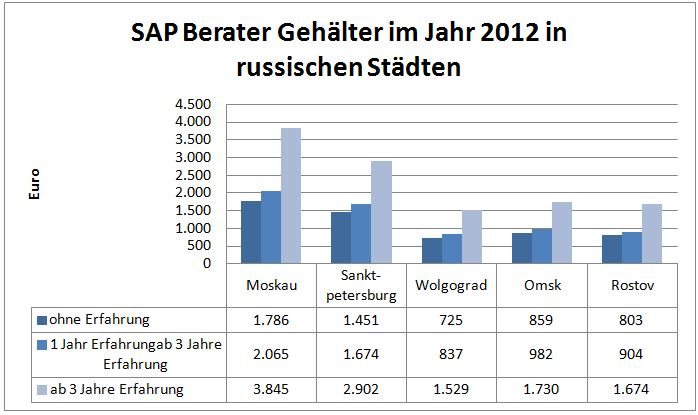
\includegraphics[width=0.7\linewidth]{./images/SAP-Berater_Gehalt_RU}
\caption{SAP-Berater Gehälter in Russland \cite{GehaltSAPBerRU}}
\label{fig:SAP-Berater_Gehalt_RU}
\end{figure}
\\
%Quelle:http://www.tadviser.ru/index.php/%D0%A1%D1%82%D0%B0%D1%82%D1%8C%D1%8F:%D0%A0%D1%8B%D0%BD%D0%BE%D0%BA_%D1%82%D1%80%D1%83%D0%B4%D0%B0_%D0%B2_%D0%A0%D0%BE%D1%81%D1%81%D0%B8%D0%B8_(%D0%98%D0%A2_%D0%B8_%D1%82%D0%B5%D0%BB%D0%B5%D0%BA%D0%BE%D0%BC)
	Ein Senior IT-Berater aus Deutschland verdient zum Vergleich durchschnittlich 6.250 € im Monat\cite{GehaltSAPBerDE}. Der Junior Berater im IT Umfeld ohne Projekterfahrung  verdient in Russland durchschnittlich 1200 € monatlich\cite{GehaltSAPBerRU}. Laut der russischen Arbeitsagentur ``rabota.ru`` steigt die Anfrage auf ERP-Systemen enorm und deswegen steigen auch die Gehälter für Spezialisten in diesem Umfeld. Die Anfänger im IT-Beratungsbereich sind beim Berufseinstieg dazu bereit fast kostenlos zu arbeiten, um wertvolle Erfahrungen im ERP-Bereich zu sammeln \cite{RusGehRabota}.
	Der deutsche Junior-Berater mit den gleichen Qualifikation und Erfahrung verdient ca. drei mal so viel (3750 €) \cite{GehaltSAPBerDE} als sein russischer Kollege.\\ \\
	\textbf{Team: %und Organisation: 
	Russisches Arbeitskollektiv gegen westlichen Team}\\
	\\
	``Das Arbeitskollektiv wurde in der sowjetischen 
	Epoche als das zentrale soziale Handlungsfeld propagiert. Es repräsentiert, dass die Geschlossenheit der Gruppe wichtiger als die Selbstverwirklichung der einzelnen Gruppenmitglieder ist. `` \cite{ProzessbeglBerRU}\\
	Gruppeninterne Konflikte blieben deshalb häufiger ungelöst oder wurden nicht diskutiert. Der Unterschied gegen dem westlichen Team besteht darin, dass russischer Kollektiv eine dauerhafte Einrichtung mit klar zugewiesenen Leitungskompetenzen ist, die vom Vorgesetzten häufig ausgeübt werden. Im Gegensatz zum russischen Kollektiv wird das westliche Team nur für die Dauer eines bestimmten Projektes eingerichtet und zeichnet sich durch die Gleichberechtigung aller Teammitglieder aus.\\
	So ein Kollektiv für Beratungszwecke ist demzufolge oft nicht flexibel und ist zu stark weisungsgebunden. Die Aufgaben im Kollektiv werden meistens vom Vorgesetzten vorgeschrieben. In unserem Fall von einem Projektleiter oder einem Manager. Solche Führungspersonen sind im IT-Beratungsfall oft an dem Büro gebunden und sind meistens in diesem Büro, während die Berater oft unterwegs bei den Kunden sind. Daher müssen die Entscheidungen intuitiv und unabhängig von dem Vorgesetzten getroffen werden. Die Tatsache, die Entscheidungen intuitiv zu treffen, spiegelt sich in dem Prinzip des russischen Kollektivs wieder.  ``Russische Organisationen zeichnen sich durch eine Konzentration von Macht auf die Führungskräfte aus. Ohne dem Vorgesetzten werden keine Entscheidungen getroffen``. \cite{ProzessbeglBerRU} \\
	Verlagerung von Entscheidungen auf die Mitarbeiter wird in Russland selten stattfinden, deswegen werden die Mitarbeiter von den Führungskompetenzen befreit und nehmen oft nur bloße Anweisungen entgegen. Für  den Beratungsprozess ist diese Tatsache ein großer Minuspunkt, weil die Berater das interdisziplinäres Wissen besitzen und  den vollen Handlungsspielraum in der IT-Beratungsbranche brauchen.
	Zu erwähnen wäre noch, dass die jungen Menschen von solcher Stereotypen weiter entfernt sind als die ältere ``sowjetische`` Generation. \\ \\
	\textbf{Gesetze: Personalauswahl und russische Gesetze}\\
	\\
	 Eine weitere wichtige Besonderheit ist die Personalauswahl. Häufig erfolgt die Auswahl von neuen Mitarbeitern nicht nach dem Kriterium der fachlichen Kompetenz. Sondern oft werden Arbeitsplätze unter Verwandten und 
	 Freunden vergeben. Es existieren fast keine etablierten Mechanismen von Angebot und Nachfrage auf dem Arbeitsmarkt. Vakanzen werden häufig nicht an den fachlich geeignetsten Bewerber vergeben, sondern an ``unseren Mann``(nash chelovek). Sinngemäße Übersetzung bedeutet, dass ``Unser Mann`` oder ```nash chelovek`` eine besondere, meist verwandtschaftliche Beziehung zum Unternehmensführer oder den Vorgesetzten des Unternehmens hat.\\
	 Ein weiteres für russische Arbeitskultur typisches Merkmal ist, dass die Gesetze, Bestimmungen und Regelungen keinen eindeutig verbindlichen Charakter haben. In Abhängigkeit von der Situation und den involvierten Personen, können Regeln oder Gesetze bewusst unberücksichtigt bleiben. Wie sich jedoch diese Abstufung darstellt ist nicht vorhersagbar. Das liegt auch daran, dass das russische Volk und die russischen Behörde sich einander nicht zutrauen. Die Strenge des Gesetzes wird oft in der Vernachlässigung der Gesetzgebung ausgeglichen. \cite{ProzessbeglBerRU}\\ \\ 
	 \textbf{Arbeitszeit, Urlaub, Work-Life-Balance}\\ %Work-life-Balance gehört dazu
	 \\
	 Die gesetzliche Wochenarbeitszeit in Russland beträgt 40 Stunden. Doch in den meisten Fällen wird diese Grenze weit überschritten. Die IT-Spezialisten arbeiten zwischen 10 und 11 Stunden am Tag in einem 5-Tage-Rhythmus \cite{ArbZeitRU}. 
	  Oft wird auch eine 6-Tage-Woche praktiziert. Zum Vergleich arbeiten deutsche IT-Berater oft weniger (siehe Kapitel-Deutschland ``Arbeitszeit und Urlaub``) und die wöchentliche Arbeitszeit der japanischen Kollegen (siehe Kapitel-Japan ``Arbeitszeit und Urlaub``) ist noch höher als in den anderen ausgewählten Ländern. 
	 In vielen Tarifverträgen in Deutschland beträgt der durchschnittliche Jahresurlaub 30 Arbeitstage. In Russland sind es dagegen nur 24 Tage. Der Arbeitstag beginnt bei russischen nicht produzierenden Firmen um 9 oder 10 Uhr \cite{ArbZeitRU}. Wenn ein IT-Berater um 10 Uhr mit seiner Arbeit beginnt, dann ist er vermutlich erst um 20-21 Uhr zu hause. Es ist dahe rzu vermuten, dass sich dies aufgrund der  hohen Arbeitszeiten auch auf private Bereiche wie Freundschaften, Familie und somit auf die Work-Life-Balance von russischen Beratern negativ auswirken könnte.   \\ 
	 Dies kann wiederum Auswirkungen auf die Arbeitsleistung und die Motivation haben.
	 \\ \\
	 \textbf{Pünktlichkeit und Reisen }\\
	 \\
	 Der IT-Berater-Beruf ist eine Tätigkeit, die mit einer höheren Reisebereitschaft verbunden ist. Beratung beinhaltet meist auch, beim Kunde vor Ort zu sein. In Deutschland sind die Berater ganz oft mit Autos unterwegs. Von einer deutschen Großstadt bis zur anderen braucht man durchschnittlich etwa 4-5 Stunden. In Russland gibt es 2 grundsätzliche Transportprobleme in Bezug auf das Consulting, die auf den Ersten Blick deutlich werden: Staus in Moskau und große Entfernungen zwischen den russischen Städten. Nachfolgend werden diese 2 Probleme näher erläutert. Das Land ist sehr groß und weit (es umfasst 11 Zeitzonen).
	 Zwischen Moskau und Nowosibirsk sind es ca. 4 Stunden nur Flugzeit plus 3 Stunden Zeitunterschied. Wenn ein Berater aus Moskau seinen Arbeitstag am Montag in Nowosibirsk beginnen möchte, muss er schon am Sonntag ausreißen. Die Reisen sind erschöpfend und werden von russischen Beratern, die z.B. eine Familie haben, nicht so gern angenommen. Für IT-Beratern mit Familie wird dadurch auch die Work-Life-Balance beeinträchtigt, da die Reisezeit gewöhnlich nicht als Arbeitszeit gewertet wird und somit von der Freizeit entbehrt werden muss.\\
	 Laut dem russischen Rating "Consulting research" aus 21 größten IT-Consulting-Unternehmen befinden sich 13 Unternehmen in Moskau\cite{RaitConsRU}.
	 Aus 100 größten russischen IT-Unternehmen befinden sich in Moskau 71 Firmen \cite{100BigITConsURU}. 
	 Moskau ist nicht nur die teuerste Hauptstadt der Welt und ein wirtschaftliches Zentrum des Landes, sondern auch ein strategischer Standort für IT-Unternehmen geworden.
	 Mit dem Wachstum der Stadt werden auch die Staus immer länger.``Nach Angaben des GPS-Navigationsanbieters TomTom ist Moskau Nummer eins unter den schlimmsten Stau-Städten der Welt\cite{MoskauStau1}.``
	 Da die Berater öfters unterwegs sind, ist es eine große Anstrengung in Moskau Auto zu fahren. Um von A nach B zu kommen wird ganz oft ein Metro benutzt. 
	 Deswegen ist es in Moskau ``erlaubt`` dem Berater sowie allen Geschäftsleuten ein Viertel bis halbe Stunde zum Meeting oder zum  Kunde zu spät zu kommen. Oft werden Staus als Ausrede, die auch akzeptiert wird, genutzt.\\
	 Allgemein zählt die Pünktlichkeit nicht zu den Stärken von Russen. Die Termine werden nicht immer eingehalten, E-Mails werden nicht sofort beantwortet und die Versprechungen sind nicht immer realistisch. Deswegen muss man als Berater diese Verzögerungen mit einplanen \cite{RusKnigge}.\\ \\
	 	 \textbf{Hierarchie und Entscheidungsfindung}\\
	 	 \\
	 Im Teilaspekt Team wurde erwähnt, dass in russischen Organisationen der Chef oder sogenannte Generaldirektor meist die alleinige Entscheidungskompetenz hat. So beschreibt auch der Sergey Frank, dass die Entscheidungskompetenzen in Russland nicht wie gewöhnt nach unten gehen, sondern nur der Geschäftsführer die Entscheidungsbefugnisse hat \cite{RuSFI}.
	 Deswegen kommunizieren die russischen IT-Berater oft nur mit dem Geschäftsführer des Unternehmens, was natürlich zur zeitlichen Verzögerungen im Projekt führen kann.\\
	 Gemäß ``Russland-Knigge`` \cite{RusKnigge} werden die Hierarchien in Russland oft  nicht eindeutig und nicht klar erkennbar. Die Berater müssen schon vor Beginn der Verhandlungen herausfinden, wer das entscheidende Wort hat. Damit wird keine Zeit durch unnötige Gespräche mit Personen, die möglicherweise keinen Einfluss auf den Verhandlungsverlauf haben, verloren.\\
	 Laut ``Businessknigge Russland`` sind ``die flachen Hierarchien nicht die Sache der Russen`` \cite{RusKnigge}. Es ist durchaus möglich, dass eine oder mehrere Personen, wie der oben beschriebene  ``nash chelovek``,  sehr viel Einfluss im Unternehmen haben, ohne dass diese einem konkreten Aufgabengebiet oder einer festen Position in der Hierarchie zugewiesen sind.\\ \\
		 	 \textbf{Lebensstandard}\\ \\
	Laut den Ergebnissen von Umfragen, die von der russischen Agentur für Finanzforschungen (russ. Abk.: NAFI) in den Jahren 2004 bis 2011 durchgeführt wurden, hat sich die materielle Lage der russischen Bürger in den vergangenen  Jahren trotz der Krise von 2008 und 2009 allmählich verbessert. \cite{LBSRu}\\
	 Die sogenannte „Vormittelklasse“, zu der fast die Hälfte aller Einwohner Russlands gehört, bestätigte einen Wachstumstrend. Dabei handelt es sich um Bürger, die genug Geld für Lebensmittel und Kleidung haben, denen jedoch der Kauf von langlebigen Waren schwer fällt. Laut der Meinungsforschung betrug diese Menschengruppe vor sieben Jahren nur höchstens 30 Prozent der Bevölkerung. In den letzten 7 Jahren ist der Anteil der armen Bürger an der Landesbevölkerung von 14 \% in 2004 auf 5\% in 2011 gesunken. Auch die Gruppe der Einwohner, denen das Geld für die Nahrungsmittel, nicht aber für die Kleidung ausreicht, ist von 35 \% in 2004 auf 28 \% in 2011 zurückgegangen. \cite{LBSRu} \\
	 Trotzdem lässt sich sagen, dass es immer noch enorme finanzielle Unterschiede zwischen der reichen und armen Bevölkerung in Russland gibt. Das durchschnittliche Gehalt in Russland beim aktuellen Währungskurs beträgt 587,60 €, in Moskau hingegen 927.57 €. Es ist noch zu erwähnen, dass die kleinen Gehälter mit dem niedrigen Lebenshaltungskosten wie gesetzliche Ausgaben, Nahrung, Kleidung usw. ausgeglichen werden. 
	\subsection*{Japan}
	\textbf{Pünktlichkeit, Kritikfähigkeit und Besonderheit der Kommunikation}\\
	\\
	Im Geschäftsleben sind die Japaner besonders pünktlich. Pünktlich bedeutet in diesem Fall 5 bis 10 Minuten vor einem Termin zu erscheinen. Selbst nur bei 5 Minuten Verspätung müssen sie an Ihren Geschäftspartner Bescheid geben, dass Sie sich verspäten. \cite{JPKnigge}. \\
	Die Kritik wird in Japan nicht direkt, sondern ausweichend und über den ``Umweg`` geäußert. Diese Kritikäußerung-Strategie wird auch von ausländischen Geschäftspartner erwartet. Eine Besonderheit in Japan hat die Bedeutung des Wortes ``Ja``. In einem Gespräch reagiert man mit ``Ja`` nicht auf die Zustimmung mit der Sache, sondern auf die Bestätigung des Zuhörers \cite{JPKnigge}. Ein lang-gesprochenes ```Ja`` bedeutet die Zustimmung vom bestimmten Sachverhalt.\\
	\\
	\textbf{Hierarchie und Rangordnung}\\
	\\
	Im japanischen Geschäftsleben spielt die Rangordnung eine wichtige Rolle.
	Beim Essen sitzt die wichtigste Person in der Mitte der Reihe. Je größer die Entfernung von ihr, desto geringer der Rang \cite{Business-KniggeFernost}.	
	Beim Meeting spricht der Ranghöchste zuerst. Bei der Begrüßung wird zuerst die Hand nicht der Frau gegeben, wie das in Deutschland üblich ist, sondern dem Ranghöchsten. \\
	\\
	\textbf{Arbeitszeit, Urlaub, Work-Life-Balance}\\
	\\
	Offiziell gilt in Japan die 40-Stunden-Woche. In der Realität sind Angestellten weit über dieses Stundenmaß hinaus bis spätabends 21 oder 23 Uhr im Büro. Wenn jemand eher nach Hause geht als sein Chef, muss er bei dem nächsten Mitarbeitergespräch mit Konsequenzen rechnen \cite{ArbZeitJP}. Den Arbeitsplatz eher als der Chef zu verlassen, zählt in Japan zu den schlechten Manieren im Geschäftsleben.
	Die Überschrift eines Online-Zeitungsartikels ``Im Japan arbeitet man sich bis zum Tode`` hat sich schon längst, und nicht unbedingt unberechtigter Weise, als japanisches Klischee etabliert. 
	16 Stunden am Tag im Büro, Schlafkammer, Mittagsschläfchen im Zug und unzählige Überstunden gehören zum modernen Arbeitsalltag in Japan. ``Schuld daran haben die Zeitarbeitsagenturen. Denn ca. ein Drittel der japanischen Arbeiterschaft besteht aus Zeitarbeitern``, sagt der amerikanische Journalist Jake Adelstein \cite{JPArbeit}. Im Gegensatz zu Deutschland, wo die Überstunden nicht immer bezahlt werden, werden in Japan die Überstunden zur zusätzlichen Geldquelle, ohne diese mancher Japaner nur schwer überleben könnte.
	Es wurde keine Quelle gefunden, um die Arbeitszeit der IT-Berater zu bestimmen. 
	In Deutschland hingegen  genießen die Arbeitnehmer 30 Tage bezahlten Urlaub. In den USA beträgt Jahresurlaub rund 2 Wochen. Offiziell sind in Japan im Durchschnitt 17 Freitage gewährt, allerdings werden nur 8 Tage im Krankheitsfall in Anspruch genommen. Weil während des Urlaubs keine Lohnfortzahlung stattfindet, muss ganz oft Urlaub unter einer Krankheit ``versteckt`` werden \cite{JPArbeitSozKultur}. Denn die Abwesenheit im Krankheitsfall wird vom Unternehmen akzeptiert und Lohnfortzahlung wird geschehen. Jedoch gibt es in Japan 16 gesetzliche Feiertage. Im Vergleich zu China mit 10 Feiertagen und Deutschland mit 20 Feiertagen, ist die Anzahl der Feiertage dafür durchschnittlich. \\
	\\
		\textbf{Gesetze: Steuer und Sozialausgaben}\\
		\\
		Steuern und Sozialabgaben sind in Japan niedriger als in Deutschland. Japanischer Mehrwertsteuer beträgt im Gegensatz zu Deutschland nur 10 \%.
		``Als Arbeitnehmer ist man in Firmen mit mehr als fünf Angestellten durch eine spezielle Krankenversicherung, einer sog. Employee Health Insurance abgesichert``. Jedoch muss man 10 bis 30 Prozent der Behandlungskosten aus eigener Tasche zahlen. Die Anteile für die Arbeitslosenversicherung übernimmt der Arbeitgeber \cite{ArbZeitJP}. \\
	\\
			\textbf{Lebensstandard}\\
			\\
		\\Der Lebensstandard in Japan ist vergleichbar mit dem mitteleuropäischen (sieh Abb.5.3).
		\begin{figure}[ht]
		\centering
		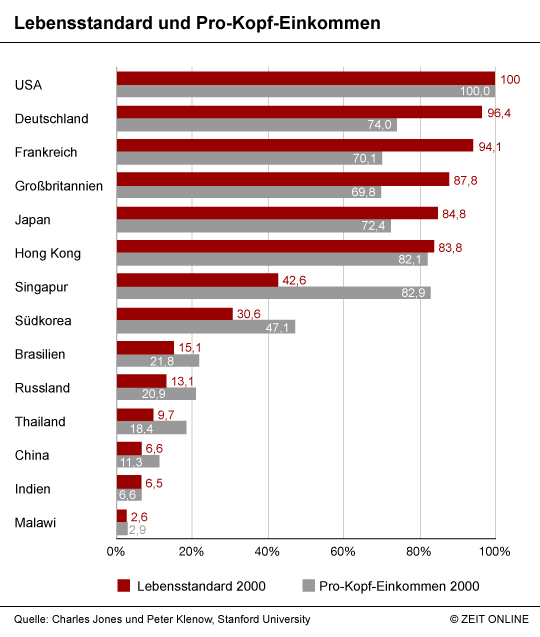
\includegraphics[width=0.7\linewidth]{./images/Lebensstandard-Pro-Kopf-Einkommen}
		\caption{Lebensstandard und Pro-Kopf-Einkommen \cite{LebensStd}}
		\label{fig:LebStdProKEink}
		\end{figure}\\
		Gemäß Miroslav Stimac sind die Ausgaben der Grundbedürfnisse in Deutschland höher als in Japan \cite[101]{Stimac2004}.
		Beispielsweise kostet Nahrung in Tokio durchschnittlich 2,36 mal mehr als in Deutschland. Viele japanische Städte leiden an Platznot, dies führt zu hohen Grundstückspreisen sowie Mietpreisen \cite[105]{Stimac2004}.
		Eine Familie mit 4 Mitgliedern im Großraum Tokio lebt oft in einer 60 qm-Wohnung \cite{ArbZeitJP}.\\	\\
		\textbf{Gehalt}\\ \\
		Das Einkommen in Japan hängt stark von dem Alter und der Betriebszugehörigkeit
		der Arbeitnehmer ab.  Laut den Angaben der Jobagentur ``CareerCross`` verdient ein japanischer IT-Berater durchschnittlich 8.000.532 Yen (56.804 €) \cite{GehaltJapan}.
		 \\ \\
			\textbf{Team}\\
			\\
		Die Bedeutung der Gruppe sowie ihr Erfolg orientiert sich, laut Michael Gehle,  nicht auf die individuellen Ziele der einzelnen Gruppenmitglieder, sondern auf einen gemeinsames Erfolg der Gruppe. Altruistisches Verhalten ist in japanischer Gesellschaft ausgeprägter als in Europa. Das Wohl des Einzelnen ist nach japanischer Auffassung vom Wohl seiner Kollegen abhängig. Mit anderen Worten bedeutet das, dass die erfolgreiche Zusammenarbeit der Gruppe eng mit der internen Zusammenarbeit der Gruppenmitglieder verbunden ist. Damit wird auch die Gruppe, ähnlich wie eine Familie betrachtet, welche Schutzfunktion übernimmt. In der nicht nur der Erfolg des gesamten Projektes, sondern auchdie Verantwortung an die Gruppenzugehörigen zu verteilen ist \cite[233]{3LaenderVergl}.\\ \\
		\textbf{Entscheidungsfindung} \\ \\
		Im Gegensatz zu Russland werden die Entscheidungsbefugnisse auch an die untere Hierarchieebene delegiert. Damit werden auch Managementanforderungen an die  Mitarbeitern niedriger Hierarchieebenen gestellt \cite[233]{3LaenderVergl}.\\
		Die Japaner haben  häufig sehr lange Entscheidungswege. Die Entscheidung wird nach top-down-Methode vom Chef angestoßen, dann verläuft die Akzeptanz der Entscheidung durch eine Organisationsspirale bis jeder Mitarbeiter diese Entscheidung wahrgenommen hat. In Deutschland wird die Entscheidungen hingegen eher formalistisch getroffen. Innerhalb des japanischen Teams gilt eine Gleichberechtigung und der Chef hat eine Rolle des Moderators. Falls während des Projektes Probleme aufgetreten sind, wird in Japan der Projektmanager häufig nicht kritisiert, sondern die Schuld wird an alle Projektmitglieder verteilt. In Deutschland dagegen trägt der Projektleiter oft die ganze Verantwortung für den Erfolg des Projektes.
%ab hier Korrektur
	\subsection*{USA}
	\textbf{Team}\\
	\\
	In der USA, sowie in Deutschland, hängt der Erfolg sowie die Karriere des einzelnen Gruppenmitgliedes, nicht so stark vom Gruppenerfolg wie in Japan ab. Laut Michael Gehle orientieren sich Karriere und Qualifizierungsmaßnahmen mehr an einzelne Mitarbeiter. Deswegen richtet sich auch deren Verhalten eher nach individuellen und nicht nach kollektiven Zielen \cite[233]{3LaenderVergl}. 
	Teamkollegen werden in der USA, sowie in westlichen Ländern, nicht selten als Konkurrenten angesehen, weil die Entlohnung an den individuellen Leistungen bemessen wird. \\ \\
		\textbf{Arbeitszeit, Urlaub, Work-Life-Balance}\\
		\\
	Die Arbeitszeit in den USA beträgt in der Regal 40 Stunden pro Woche. 
	Ein Drittel aller US-Amerikaner arbeiten länger als 40 Stunden pro Woche.
	Laut der UN-Studie arbeiten US-Angestellte im Durchschnitt etwa 500 Stunden mehr als deutsche Arbeitnehmer \cite{ArbeitsumgUSA}. Die meisten US-Amerikaner haben nur 10 bezahlte Urlaubstage \cite{InfoUSArbVertr}.\\ \\
	\textbf{Gesetze: Besonderheiten in Arbeitsgesetzen}\\
		\\
		Die Lohnfortzahlung im Krankheitsfall beträgt in den USA nur 7 Tage pro Jahr. 
		Mitarbeiter im IT Bereich haben häufig keinen Anspruch auf Überstundenausgleich. Man kann allerdings häufig aber inoffiziell einen zusätzlichen Tag in der Woche frei nehmen, um die Überstunden auszugleichen. Als Überstundenausgleich dient auch am Ende des Jahres ein finanzieller Bonus \cite{InfoUSArbVertr}.
		Solche Vereinbarungen sind jedoch nicht gesetzlich geregelt und müssen zusätzlich werden.\\
		Die Kündigungsfrist beträgt, sowohl für Arbeitgeber als auch für 
		Arbeitnehmer, zwei Wochen. Aufgrund der kurzen Kündigungsfrist gibt es in den USA keine Probezeit.\\
		Im ersten Arbeitsjahr gibt es in den USA keinen Anspruch auf Urlaub. \cite{USA_Tipps}.
		\\ \\
	\textbf{Gehalt}\\
		\\
		Laut Firma ``indeed`` beträgt das Jahresgehalt des IT-Beraters (Technical Consultant`s in USA) rund 86.000 \$ (sieh Abb. 5.4).
		\begin{figure}[ht]
				\centering
				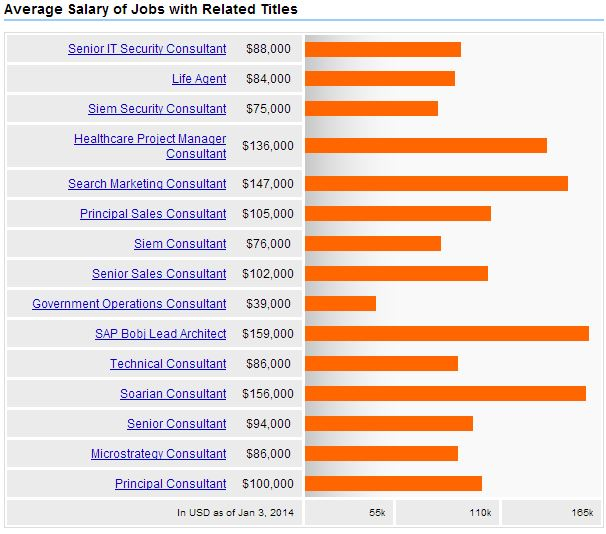
\includegraphics[width=0.7\linewidth]{./images/Techn_Cons_Sal}
				\caption{Jahresgehalt von IT-Consultants in USA}
				\label{fig:TechConsSal}
				\end{figure}\\
				%Wo ist Quelle???
		``Ein europäisches Gehalt in EUR ist ungefähr 1:1 vergleichbar mit einem 
		amerikanischen Gehalt in USD. Es wäre nicht richtig, den offiziellen Umrechnungskurs anzusetzen, da die Lebenshaltungskosten in USD in den USA mit den Lebenshaltungskosten in EUR in Europa vergleichbar sind`` \cite{InfoUSArbVertr}. In der IT-Branche wird oft ein Provision angeboten, die vom Erfolg des
		Projektes abhängt. Das Gehalt wird in zwei Raten ausbezahlt, in der Regel am 15. und am letzten Tag des Monats.\\ \\
	\textbf{Hierarchie} \\ \\
	Gemäß US-Internetportal ``hierarchystructure.com`` \cite{HierarchieUSA} gehört die US- Geschäftshierarchie zu den erfolgreichsten Geschäftshierarchien der Welt und wird von vielen Ländern als Vorbild gesehen, um wirtschaftliches Wachstum zu erzielen. Geschäftsstruktur und Hierarchie einer Organisation werden mit dem Zweck das Gruppenziel zu erreichen aufgebaut, wobei jeder einzelne Mitglied der Organisation unterstützt wird. Dabei werden die Positionen, Aufgaben und zugehörigen Mitarbeiterrollen klar definiert.
\begin{figure}[ht]
\centering
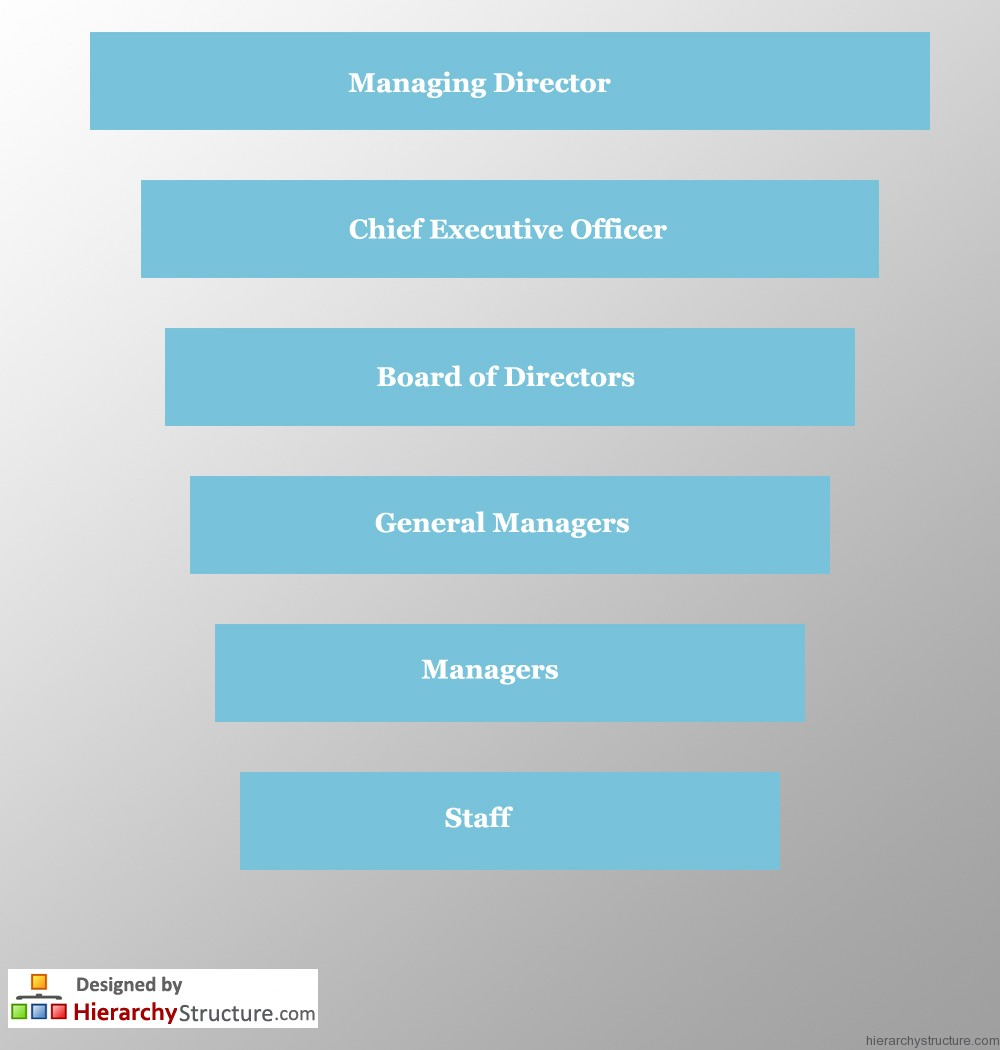
\includegraphics[width=0.7\linewidth]{./images/USA-Business-Hierarchy}
\caption{Geschäftshierarchie USA \cite{HierarchieUSA}}
\label{fig:USA-Business-Hierarchy}
\end{figure}

	\subsection*{Deutschland}
	In allen beschriebenen Ländern unterscheidet sich der Formalisierungsgrad der Arbeitskultur erheblich. In Deutschland werden Verhaltensweisen und Standards der Arbeitskultur sehr formalisiert und in Form von gesetzlichen Vorschriften definiert. Dies führt zu einer starken Bürokratie. In Japan weist die Arbeitskultur auch einen hohen Formalisierungsgrad auf. Das hat jedoch weniger mit gesetzlichen Regelungen wie in Deutschland, sondern eher mit traditionellen Verhaltensweisen zu tun \cite[236]{3LaenderVergl}. Es gibt noch 2 weiteren Eigenschaften, welche die deutsche Arbeitskultur charakterisieren. Dazu zählen sehr direkte Kommunikation und die gründliche Planung.\\ \\
	\textbf{Pünktlichkeit}\\ \\
	Pünktlichkeit, sowie gründliche Planung, gehören zu den Stärken der Deutschen. IT-Consultants sind oft keine Ausnahme. Die Termine sollen gründlich geplant werden, bevor man zur Verhandlung kommt. Natürlich müssen die Termine zeitlich eingehaltenen werden. Es wird bei der Planung meist eine Pufferzeit eingerechnet, falls es trotz der aufwändigen Planung zu den zeitlichen Verzögerungen kommen soll.\\ \\
	\textbf{Team} \\ \\
		Auch die  Trennung zwischen dem privaten und beruflichen Leben, zeichnet die  deutsche Arbeitskultur aus. Im Gegensatz zu China oder Russland, wo das Arbeitsteam oft als 2. Familie eingesehen ist, hat Deutschland an dieser Stelle einen formalistischen Charakter. Trotz allem was ein Team zusammen erlebt, heißen Teammitglieder unter einander ``Arbeitskollegen``. Laut ``Germany Trade and Invest``
		Gesellschaft für Außenwirtschaft und Standortmarketing sind Einladungen  von Geschäftspartner für private Aktivitäten in Deutschland eher selten, sofern die  Geschäftsbeziehungen nicht schon sehr lange bestehen \cite{ArbKulturDE}. Ob diese Tatsache eine besondere Auswirkung auf Beratungsgeschäft hat, ist nicht leicht differenzierbar. An dieser Stelle besteht ein Bedarf zur Forschung. \\ \\
	\textbf{Arbeitszeit, Urlaub, Work-Life-Balance } \\ \\
	Wie schon im Russland-Kapitel erwähnt wurde, beträgt die gesetzlich geregelte Arbeitszeit in Deutschland 40 Stunden pro Woche. Montags bis Donnerstags sind die IT-Berater oft beim Kunde vor Ort und zeitlich sehr ausgelastet. Das hat damit zu tun, dass die Berater, wenn sie schon beim Kunde sind, versuchen möglichst viele Probleme zu lösen. Das führt nicht selten zu den Überstunden, die am Freitag entweder durch ein Meetings-Tag im Büro oder ein Selbststudium-Tag im Home-Office kompensiert werden. Am Freitag werden beispielsweise auftretende Probleme während des Beratung analysiert und neue Lösungen vorgeschlagen. Die Work-Life-Balance, was bei vielen Unternehmen heutzutage das Modethema ist, entspricht meistens nicht den Erwartungen der Junior-Berater \cite{JNRBer}. 
	Manche IT-Beratungsfirmen, meistens Großunternehmen, verteilen die Projekte nach einem Senioritätsprinzip. Das bedeutet, dass ältere Berater oder die Berater, die länger im Unternehmen sind und eine Familie besitzen, öfter in den lokalen Projekten tätig sind. Damit wird oft erreicht, dass solche Berater mehr Zeit für Freunde oder Familie haben, indem sie nicht so oft reisen, wie die anderen und sogar eine Möglichkeit haben in der Woche zu Hause übernachten.\\
	Der Arbeitstag beginnt in Deutschland im Vergleich zu den anderen Ländern wie in Russland, wo die meisten Büros erst ab 10 Uhr geöffnet sind, sehr früh. Bürozeiten ab 7 Uhr sind keine Seltenheit \cite{ArbKulturDE}. %Dieser Rhythmus wurde für meisten IT-Berater sehr gut eignen, weil man wegen der Einbindung an vielen Personen, alle    
	
	\textbf{Gehalt} \\ \\
	Die Gehälter der deutschen IT-Berater werden von vielen Faktoren beeinflusst. Dazu zählen die Größe, Branche und Region des Unternehmens, sowie die Noten des Studienabschlusses, das Tätigkeitsfeld, individuelle Fähigkeiten des IT-Consultants und andere Faktoren. Allgemein werden die IT-Berater sehr gut bezahlt. IT-Projektleiter, IT-Sicherheitsexperte, sowie IT-Berater verdienen am besten im deutschen IT-Umfeld \cite{VerdienstITinDE}.\\
	Senior IT-Berater aus Deutschland verdienen durchschnittlich 6.250 € monatlich. Der deutsche Junior-Berater ohne Erfahrung in der Beratungsbranche verdient ca. 3750 € im Monat .\cite{GehaltSAPBerDE} \\
	Die deutschen Berater, die ins Ausland geschickt werden, haben eine separate Vergütung über das gesetzliche Tagesgeld.\\ \\
	\textbf{Lebensstandard} \\ \\
	Laut der Rangliste für den Lebensstandard und Pro-Kopf-Einkommen von Jones und Klenow, die im Jahr 2010 für 134 Staaten veröffentlicht wurde, steht Deutschland auf dem 2. Platz nach der USA (sieh Kapitel Japan - Gesetze: Steuer und Lebensstandard \label{LebStdProKEink}). Trotz dieser Rangliste sinkt der Lebensstandard in Deutschland seit Euro-Einführung immer noch. Im Vergleich zu den südeuropäischen Ländern wie Portugal oder Spanien, müssen die Kernstaate der EU, zu denen z.B. Deutschland gehört, deutliche Verluste, nicht nur am Einkommen, hinnehmen. \cite{SteigungDELebstd}.\\
	Um sich einen detaillierteren Eindruck zu verschaffen, ist es wichtig die Faktoren, welche den Lebensstandard  der deutschen Bevölkerung maßgeblich beeinflussen, zu bestimmen. Gemäß dem Online-Statistikportal statista, sind folgende Dinge (sieh Abb. 5.6) zu leisten, damit man einen akzeptablen Mindestlebensstandard in Deutschland hat.

\begin{figure} [hp]
\centering
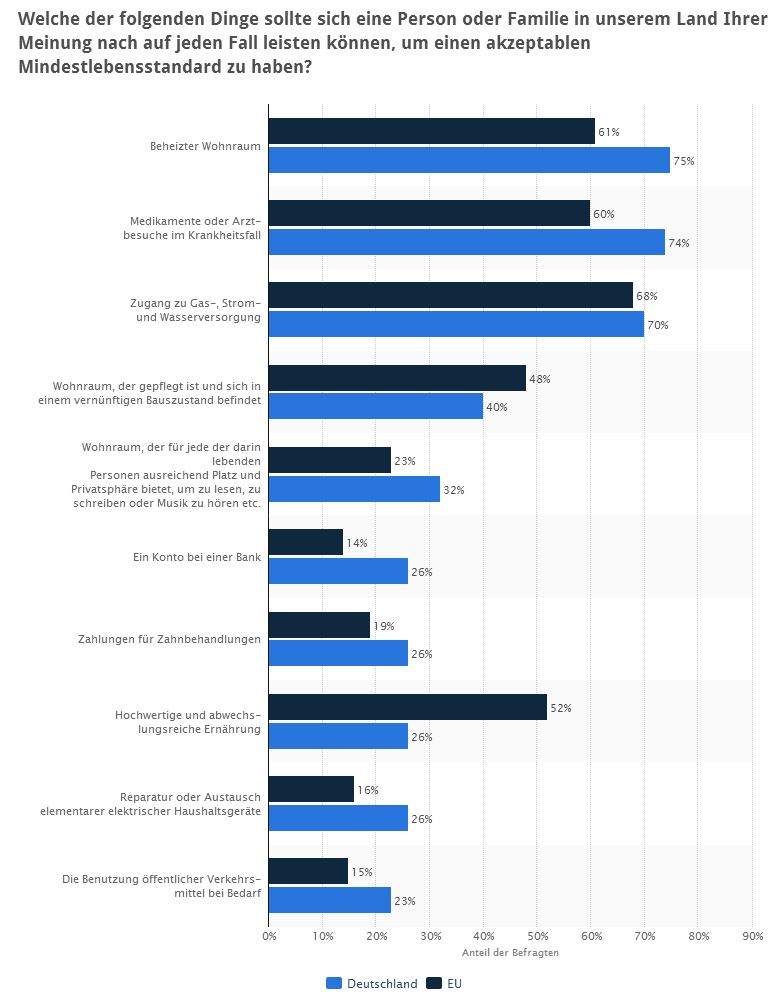
\includegraphics[width=0.7\linewidth]{./images/FaktorenLebensstand}
\caption{Faktoren des Lebensstandards in Deutschland \cite{statistaDeLebnst}}
\label{fig:FaktorenLebensstand}
\end{figure}
%\textbf{Hierarchie}
\newpage
\section{Abschluss und Vergleich}
Zum Schluss vergleichen wir einige Teilaspekte und signifikante Indikatoren der ausgewählten Länder, um Rückschlüsse auf die Arbeitskultur im IT-Beratungsgeschäft zu ziehen.
%\begin{table}[htp]
%\begin{tabular}{|c|c|c|c|c|c|}
%\hline  Aspekt/Land& Deutschland & USA & Russland & Japan & Indien \\ 
%\hline 	Hierarchien  & z & ja & ja & ja &  z \\ 
%\hline  Gehalt& ja & ja & ja & ja & z \\ 
%\hline  Gesetze& z & ja & ja & ja & z  \\ 
%%\hline  Grad des intuitiven Handelns& ? & ? & ? & ? & ? & ? \\ 
%\hline  Kritikfähigkeit& z & z & z & ja & z \\ 
%\hline  Team& ja & ja & ja & ja & z\\ 
%\hline  Entscheidungsfindung& x & x & ja & ja & z  \\ 
%\hline  Lebensstandard& ja & ja & ja & ja & z \\ 
%\hline  Pünktlichkeit& ja & z & ja & ja & z\\ 
%\hline  Arbeitszeit, Urlaub, W-L-B& ja & ja & ja & ja & z\\ 
%\hline 
%\end{tabular} 
%\caption{Matrix der Arbeitskultur 2}
%\end{table}	\\
%Um die überarbeitete Matrix richtig verstehen zu können, muss man zuerst die einzelnen Symbole definieren. Das Symbol ``Ja`` bedeutet, dass die Information über dem Teilaspekt bezüglich der IT-Beratung im internationalem Kontext vorhanden war und man daraus einen Vergleich über den gleichen Teilaspekt in ausgewählten Ländern machen kann. Das ``x`` bedeutet, dass man entweder die Information nicht vollständig hat oder, dass es keine eindeutige Beziehung zum unseren Thema gibt. Beispielsweise gibt es genug Information zu den deutschen Gesetzten, trotzdem gibt es hier keine Besonderheit, die den Beratungsprozess in maßgeblicher Weise beeinflusst. Das ``z`` bedeutet, dass aus zeitlichen Gründen keine Information gefunden wurde. Dazu gibt es mehrere Gründe wie bspw. die zeitliche Begrenzung des Projekts, sowie knappe Ressourcen in Form von Projektmitgliedern. Ein weiterer Grund besteht darin, dass es wichtiger war,  Prioritäten zu setzen und die Teilaspekte mit erhöhter Relevanz detaillierter zu betrachten.\\ \\
Ein wichtiger Teilaspekte ist das Gehalt der IT-Berater. Wenn wir die Gehälter von den Senior-Berater in den ausgewählten Ländern vergleichen, dann kann man vermutlich sagen, dass die Senior-IT-Berater aus Deutschland am meisten verdienen.
\begin{table}[htp]

\begin{tabular}{|c|c|c|c|c|}
\hline Land & Deutschland & USA & Japan &  Russland\\ 
\hline durch. Gehalt in € & 75.000 & 63.537 & 56.804 &  46.140\\ 
\hline 
\end{tabular} 
\caption{IT-Berater-Gehälter in ausgewählten Ländern}
\end{table}

Wenn wir das Gehalt in Beziehung mit dem Lebensstandard	in diesen Ländern betrachten. Dann können wir vermuten, dass die Lebenshaltungskosten in Russland  geringer sind als in Deutschland. Wenn wir das Gehalt und Lebensstandard ins Verhältnis setzen, dann ergibt sich ganz andere Gehälter-Ranking: Russland > Deutschland > USA > Japan.
\begin{figure}[ht]
		\centering
		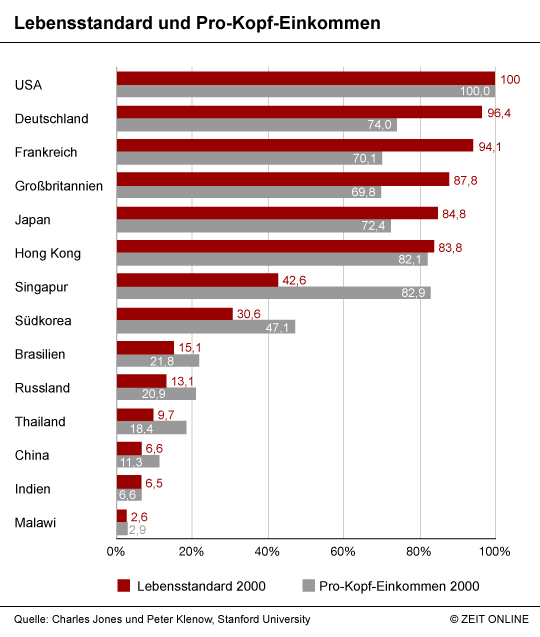
\includegraphics[width=0.7\linewidth]{./images/Lebensstandard-Pro-Kopf-Einkommen}
		\caption{Lebensstandard und Pro-Kopf-Einkommen \cite{LebensStd}}
		\label{fig:LebStdProKEink}
		\end{figure}
Wenn unsere Vermutungen richtig sind, dann arbeiten IT-Berater aus Japan mit Abstand am meisten. Im Allgemeinen arbeiten IT-Berater in allen ausgewählten Ländern mehr als der Durchschnitt. Der Grund liegt an dem Beruf des Beraters und seinen spezifischen Eigenschaften wie Kundennähe, Reisebereitschaft usw. Um eine gute Work-Life-Balance zu erreichen, müssen Berater viel Selbstdisziplin haben, um die private Zeit ordentlich zu verwalten.\\
Wenn wir den Aspekt ``Gesetze`` betrachten, dann können wir abschließend sagen, dass es einige interessante Fakten in den ausgewählten Ländern gibt. Steuern und Sozialabgaben sind in Japan beispielsweise geringer als in Deutschland. In den USA gibt es Besonderheiten im Arbeitsgesetz. Es gibt keine Kündigungszeit aufgrund der kleinen Probezeit. In Russland gibt es eine Besonderheit bei der Personalauswahl(``unser Mann``) und die Gesetze haben meistens keinen eindeutig verbindlichen Charakter.\\
Wenn wir den Aspekt Team analysieren, dann kann man nachträglich sagen, dass einige Besonderheiten bei der Gruppenarbeit im Beratungsgeschäft in diesen Ländern gibt. In Russland, sowie in Japan wird das Team, in diesem Fall passt der Begriff ``Arbeitskollektiv`` am besten, von den historischen und kulturellen Eigenschaften des Volkes stark beeinflusst. Im Gegensatz zu diesen beiden Ländern, gibt es in den westlichen Ländern wie Deutschland und den USA eher ein modernes Team mit der Gleichberechtigung aller Teammitglieder.\\
Abschließend lässt sich sagen, dass es sehr wichtig war, den Aspekt der Arbeitskultur für den internationalen Beratungsprozess zu analysieren und zu vergleichen. Denn die Arbeitskultur beeinflusst nicht nur das Geschäftsleben von IT-Berater,, sondern auch deren Privatsphäre. Es hat sich auch viele Unterschiede sowie einige Gemeinsamkeiten zwischen ausgewählten Ländern bezüglich der Arbeitskultur im IT-Beratungsgeschäft herauskristallisiert. Es gab auch einige interessante Fakten, die für IT-Berater gut zu wissen sind, falls sie international agieren. Das wichtigste an dieser Stelle ist noch mal zu sagen, dass man die fremde Arbeitskultur als IT-Berater im internationalen Umfeld nicht unterschätzen soll.






%neu Matrix-die ausgefüllt wird, mit umformulierten Teilaspekten. Begrüdnung:
%Durch einer Recherchewerden einige Teilaspekte verändert. Dafür gibt es mehrere Gründe, bspw. waren die recherchierten Teilaspekte besser formuliert oder einige waren in ihrer Definition zu weit gefasst und müssten demzufolge zusammengefasst werden. Für bestimmte Teilaspekte gibt es keine Information, die durch Recherche in 3 verschiedenen Sprachen (Deutsch, Englisch und Russisch) nicht zu finden ist. An dieser Stelle besteht noch Forschungsbedarf. \\
%1)Hierarchien->Hierarchien(plus Organisation) 2)Kundenverh weg 3)spezielle Rechtslage->Gesetze 4)Grad des intuitiven Handelns weg 5) Kritikfähigkeit nur bei Japan,De 6) Lebensumstände ->Lebensstandards ->Zeitmanagement in Form von Pünktlichkeit 7)Work-Life-Balance-> Arbzeit und Urlaub(Work-Life-Balance wird ersichtlich) 8)tagesrythmus gehört zur Arbeitszeit und Urlaub
